%%
%% This is file `sample-xelatex.tex',
%% generated with the docstrip utility.
%%
%% The original source files were:
%%
%% samples.dtx  (with options: `sigconf')
%% 
%% IMPORTANT NOTICE:
%% 
%% For the copyright see the source file.
%% 
%% Any modified versions of this file must be renamed
%% with new filenames distinct from sample-xelatex.tex.
%% 
%% For distribution of the original source see the terms
%% for copying and modification in the file samples.dtx.
%% 
%% This generated file may be distributed as long as the
%% original source files, as listed above, are part of the
%% same distribution. (The sources need not necessarily be
%% in the same archive or directory.)
%%
%% The first command in your LaTeX source must be the \documentclass command.
\documentclass[sigconf]{acmart}

%%
%% \BibTeX command to typeset BibTeX logo in the docs
\AtBeginDocument{%
  \providecommand\BibTeX{{%
    \normalfont B\kern-0.5em{\scshape i\kern-0.25em b}\kern-0.8em\TeX}}}

%% Rights management information.  This information is sent to you
%% when you complete the rights form.  These commands have SAMPLE
%% values in them; it is your responsibility as an author to replace
%% the commands and values with those provided to you when you
%% complete the rights form.
\setcopyright{acmcopyright}
\copyrightyear{2020}
\acmYear{2020}
\acmDOI{10.1145/1122445.1122456}

%% These commands are for a PROCEEDINGS abstract or paper.
\acmConference[Woodstock '18]{Woodstock '18: ACM Symposium on Neural  Gaze Detection}{June 03--05, 2018}{Woodstock, NY}
\acmBooktitle{Woodstock '18: ACM Symposium on Neural Gaze Detection,
  June 03--05, 2018, Woodstock, NY}
\acmPrice{15.00}
\acmISBN{978-1-4503-XXXX-X/18/06}


%%
%% Submission ID.
%% Use this when submitting an article to a sponsored event. You'll
%% receive a unique submission ID from the organizers
%% of the event, and this ID should be used as the parameter to this command.
%%\acmSubmissionID{123-A56-BU3}

%%
%% The majority of ACM publications use numbered citations and
%% references.  The command \citestyle{authoryear} switches to the
%% "author year" style.
%%
%% If you are preparing content for an event
%% sponsored by ACM SIGGRAPH, you must use the "author year" style of
%% citations and references.
%% Uncommenting
%% the next command will enable that style.
%%\citestyle{acmauthoryear}

%%
%% end of the preamble, start of the body of the document source.
\begin{document}

%%
%% The "title" command has an optional parameter,
%% allowing the author to define a "short title" to be used in page headers.
\title{State of the Art Report - Crowd Simulation}

%%
%% The "author" command and its associated commands are used to define
%% the authors and their affiliations.
%% Of note is the shared affiliation of the first two authors, and the
%% "authornote" and "authornotemark" commands
%% used to denote shared contribution to the research.
\author{Manuel Eiweck}
\affiliation{
	\institution{Student of Technical University Vienna}
}
\email{e1633012@student.tuwien.ac.at}

%%\author{Bernhard Kerbl}
%%\affiliation{
%%	\institution{Institute of Visual Computing \& Human-Centered Technology, Technical University Vienna}
%%}
%%\authornote{Advisor}
%%\email{kerbl@cg.tuwien.ac.at}

%%
%% By default, the full list of authors will be used in the page
%% headers. Often, this list is too long, and will overlap
%% other information printed in the page headers. This command allows
%% the author to define a more concise list
%% of authors' names for this purpose.
\renewcommand{\shortauthors}{Manuel Eiweck}

%%
%% The abstract is a short summary of the work to be presented in the
%% article.
\begin{abstract}
The goal of this state of the art report is to give a quick overview of the topic. Reader should be able to understand what application areas and research areas are covered, important key concepts and technical terms often used in the field. As crowd simulation is a broad field it is not possible to cover all approaches to a given problem, so there are additional references for further detailed reading. 

In the Introduction key areas, common definitions and terms as well as first research results done in the field are explained. The Report continues with common application areas and an overview of the research areas and the problem these try to solve. After that each area is described in more detail with given approaches. At the end there is a outlook for future research necessary in crowd simulation. 
\end{abstract}

%%
%% The code below is generated by the tool at http://dl.acm.org/ccs.cfm.
%% Please copy and paste the code instead of the example below.
%%
\begin{CCSXML}
<ccs2012>
<concept>
<concept_id>10010147.10010371.10010352</concept_id>
<concept_desc>Computing methodologies~Animation</concept_desc>
<concept_significance>500</concept_significance>
</concept>
<concept>
<concept_id>10010147.10010371.10010352.10010381</concept_id>
<concept_desc>Computing methodologies~Collision detection</concept_desc>
<concept_significance>500</concept_significance>
</concept>
<concept>
<concept_id>10010147.10010371.10010352.10010379</concept_id>
<concept_desc>Computing methodologies~Physical simulation</concept_desc>
<concept_significance>100</concept_significance>
</concept>
<concept>
<concept_id>10010147.10010371.10010352.10010378</concept_id>
<concept_desc>Computing methodologies~Procedural animation</concept_desc>
<concept_significance>500</concept_significance>
</concept>
<concept>
<concept_id>10010147.10010341.10010370</concept_id>
<concept_desc>Computing methodologies~Simulation evaluation</concept_desc>
<concept_significance>300</concept_significance>
</concept>
<concept>
<concept_id>10010147.10010341.10010349.10010359</concept_id>
<concept_desc>Computing methodologies~Real-time simulation</concept_desc>
<concept_significance>500</concept_significance>
</concept>
<concept>
<concept_id>10010147.10010341.10010349.10010362</concept_id>
<concept_desc>Computing methodologies~Massively parallel and high-performance simulations</concept_desc>
<concept_significance>500</concept_significance>
</concept>
</ccs2012>
\end{CCSXML}

\ccsdesc[500]{Computing methodologies~Animation}
\ccsdesc[500]{Computing methodologies~Collision detection}
\ccsdesc[100]{Computing methodologies~Physical simulation}
\ccsdesc[500]{Computing methodologies~Procedural animation}
\ccsdesc[300]{Computing methodologies~Simulation evaluation}
\ccsdesc[500]{Computing methodologies~Real-time simulation}
\ccsdesc[500]{Computing methodologies~Massively parallel and high-performance simulations}

%%
%% Keywords. The author(s) should pick words that accurately describe
%% the work being presented. Separate the keywords with commas.
\keywords{crowd simulation, state of the art report}

%% A "teaser" image appears between the author and affiliation
%% information and the body of the document, and typically spans the
%% page.
\begin{teaserfigure}
  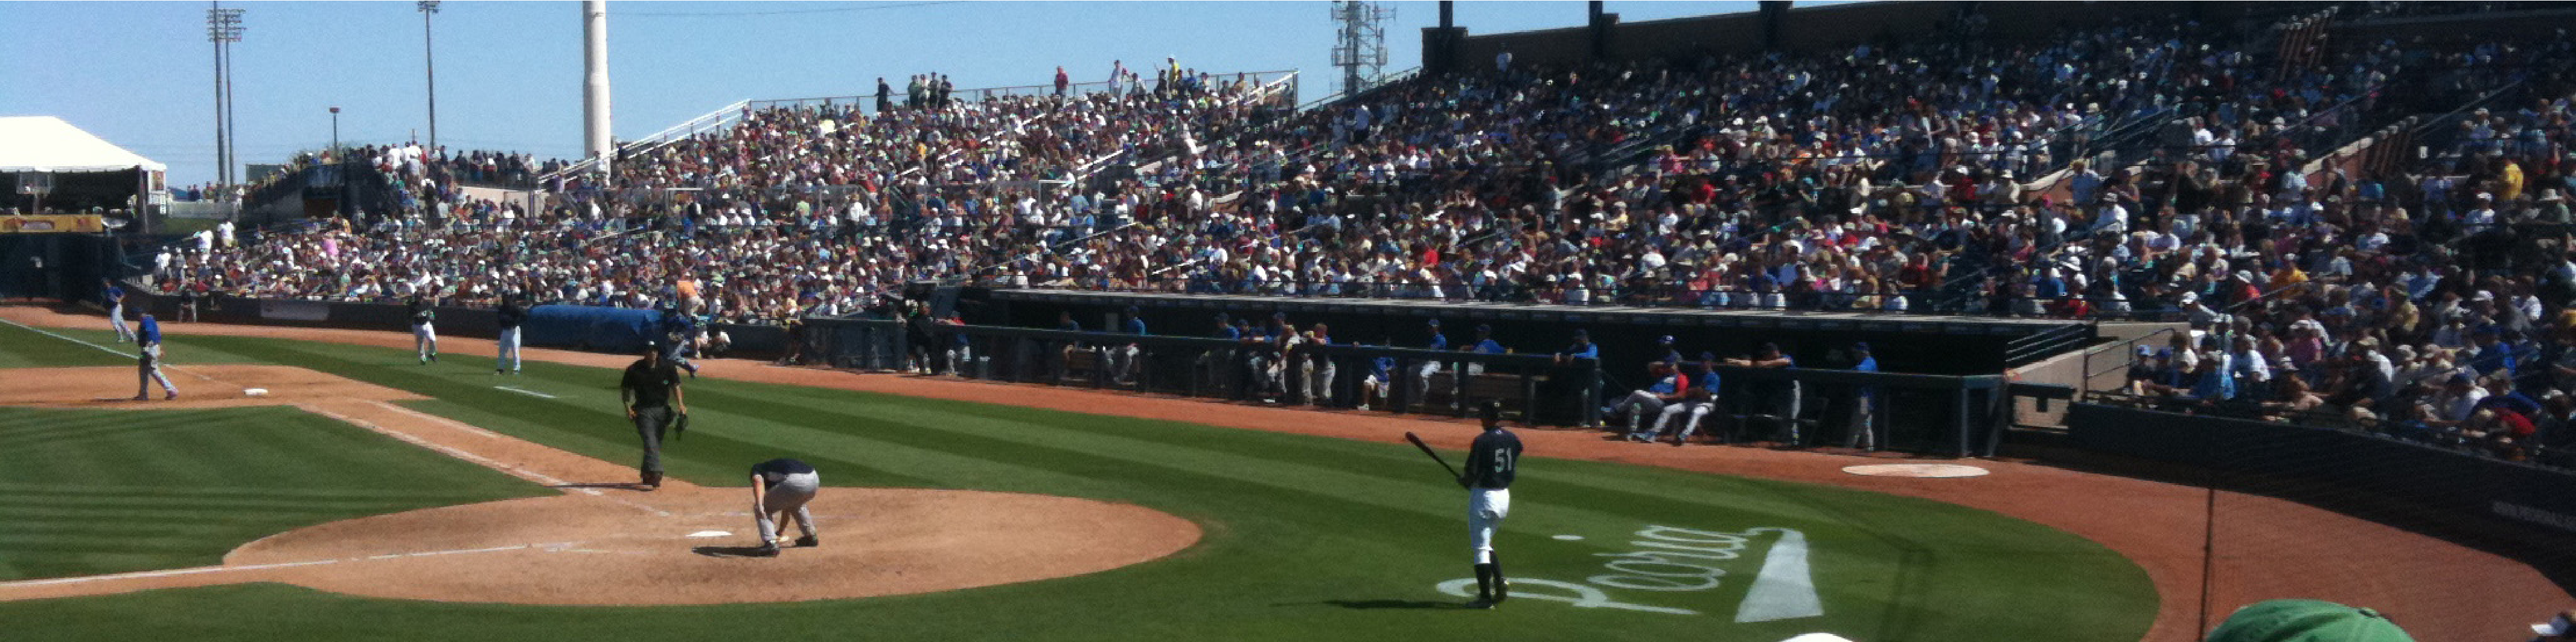
\includegraphics[width=\textwidth]{sampleteaser}
  \caption{Seattle Mariners at Spring Training, 2010.}
  \Description{Enjoying the baseball game from the third-base
  seats. Ichiro Suzuki preparing to bat.}
  \label{fig:teaser}
\end{teaserfigure}

%%
%% This command processes the author and affiliation and title
%% information and builds the first part of the formatted document.
\maketitle

\section{Introduction}

A good comprehensive work on crowd simulation is the book "Crowd Simulation" \cite{thalmann_crowd_2013} in the introduction part I will sum up some key aspects. 

At the beginning some information for the research field in general. The research results in crowd simulation does not come from one or two specific scientific fields or communities, rather the results is a combination of many different fields. A big part comes from the computer graphics field but there is also research done in architecture, physics, robotics, safety science, sociology and so on(TODO: zitat zu werken von den bereichen). A resulting problem is that it is difficult to keep up to date with the current research and because each science field uses different publication methods it is especially easy to overlook some papers on different fields and miss usefully information for the own research. In addition most papers are presenting an solution to a specific problem, for example a pedestrian simulation in real time \cite{karamouzas_predictive_2009},which is not very useful when you want to simulate a big fighting scene in a movie.


\subsection{Key areas}
\label{chap:key_areas}
For a believable crowd simulation there are two parts. First we need to have \textbf{"behavioral animation and environment modeling"}\cite{thalmann_crowd_2013} which defines how the crowd is moving and reacting to each other and the environment. Some example research papers here are for example "Flocks, herds and schools: A distributed behavioral model"\cite{reynolds_flocks_1987} or "Social force model for pedestrian dynamics"\cite{helbing_social_1995}. Second we also need \textbf{"crowd rendering"}\cite{thalmann_crowd_2013} for displaying the large amount of agents in the crowd, where performance is especially important in real time simulations. Crowd rendering also researches the level of detail we are rending, a evacuation simulation could use points or a simple 3D model of a person on the other hand a simulation for movies or games would need more details. Here some examples would be "TODO".

Most application on crowd simulation focus on one of two key areas: 
\begin{itemize}
\item \textbf{"Realism of behavioural Simulation"}\cite{thalmann_crowd_2013} keywords: crowd dynamic, evacuation simulation, social models, collision avoidance and evaluation of results to the real world
\item \textbf{"High quality rendering"}\cite{thalmann_crowd_2013} keywords: crowds in movies and games, performance optimization, combination with motion capturing and physics simulation  
\end{itemize}

\cite{thalmann_crowd_2013}

\subsection{Simulation Models}

To simulate realistic crowd behavior a model is needed which specifies how the crowd reacts in each simulation step. The used models can be classified in roughly two groups macroscopic and microscopic models. The difference is how they see an agent in a crowd. An \textbf{agent} is a single actor in a crowd simulation which can move and act independently from other agents, this can be a human in a crowd of people but also a car in a traffic simulation. However on some applications and paper especially those who handle real time simulations agents are grouped to reduce the simulation cost and only rendered as multiple agents / persons, an example are the "TotalWar" \cite{total_war_website} \cite{thalmann_crowd_2013} game series.

\subsubsection{\textbf{macroscopic models}}
These types of models try to simulate the crowd as an whole unit, they are often used in a real-time scenario because the number of individual agents in the crowd does not highly affect performance in the simulation. In some papers they are also referred as "continuum-based"\cite{xu_crowd_2014}. The goal here is that the crowd as a whole reacts realistically. These simulation can be compared to gas or fluid simulations, because there is not each particle or in our case each agent simulated moreover there is a common path for the fluid or whole crowd simulated. An example are the pedestrian and crowd simulation papers from Hudges \cite{hughes_continuum_2002} \cite{hughes_flow_2003}

\subsubsection{\textbf{microscopic models}}
On the other hand microscopic models, also referred as "agent-based"\cite{xu_crowd_2014} try to simulate each single agent. The resulting simulation often brings better results than a simulation with a macroscopic model but it also costs more performance, so it is not suitable for simulating large crowds in real time. Most approaches define rules for each agent how to react to the environment and different scenarios. There is a lot of different papers and approaches which rules and attributes provide what results. A common used approach is force-based, famous cited papers are "Social force model for pedestrian dynamics" \cite{helbing_social_1995} and "Flocks, herds and schools: A distributed behavioral model" \cite{reynolds_flocks_1987}. TODO: insert other paper references from xu crowd 2014 2.2 .A often resulting problem is that "agents appear to shake or vibrate in high-density crowds"\cite{xu_crowd_2014}

\cite{xu_crowd_2014}\cite{thalmann_crowd_2013}

\subsection{crowd rendering overview}
TODO
\subsection{elementary papers}
In the following section i want to sum up some often cited and elementary papers for crowd simulation. 
\subsubsection{Flocks, herds, and schools: A distributed behavioral model.}\cite{reynolds_flocks_1987}
is one of the most famous first published papers for the field. The paper describes an approach for modeling a simulation of a flock of birds and other crowds. At that time the common way to simulate a crowd would be to script the path of each agent individually. Reynolds defined some key concepts and keywords for the crowd simulation field for example he introduced the idea of what later would become known as agend-based or microscopic simulation:
\begin{quote}
"Yet all evidence indicates that flock motion must be merely the aggregate result of the actions of individual animals, each acting solely on the basis of its own local perception of the world. (...) This approach assumes a flock is simply the result of the interaction between the behaviors of individual birds. To simulate a flock we simulate the behavior of an individual bird (...)"
\end{quote}
He also compares his approach to a particle system for simulating dynamic "fuzzy objects", but the differences in his approach is that each particle/bird has a complex geometrical state (orientation, animation for example flight banking) and that a bird flock is more complex to describe than other particle systems like a fire for example in addition basic particle systems do not simulate the interaction between the particles.  
\begin{quote}
"Boid behavior is dependent not only on internal state but also on external state"
\end{quote}
He defines the \textbf{actor} as "computational abstraction that combines process, procedure, and state." This is still relevant because most microscopic simulation approaches use a similar concept for abstracting the simulation system from the actual application, here a bird flock.  
In addition there is also a chapter on how flocks are interacting with another. An interesting statement is: 
\begin{quote}
"birds can flock with any number of flockmates because they are using what would be called in formal computer science a constant time algorithm. "
\end{quote}
The reason for this is that the birds does not include all other individual birds for their decision making, instead they only rely on itself, the nearest neighbors and a filtered perception on the rest of the flock. This  filtering of  information is also seen on other papers which cover level of detail in crowd simulations \cite{osullivan_levels_2002}. Of course in a simulation there will be a limit for a maximum of individual agents. 

The paper continues with more information about the aspects of what to consider when rendering crowds with the example of the bird flock and other animal crowds. Many of these aspects and problems are still relevant in current papers that is the reason why this an important elementary paper in the crowd simulation field, however when it comes to details in the implementation of the algorithm there are more up to date approaches. 

\subsubsection{Social force model for pedestrian dynamics}\cite{helbing_social_1995} is an important paper when it comes to pedestrian simulation for common daily tasks, these crowd flow simulations are used in the architectural field in planning state for large buildings train station, airports, shopping centers etc.. 
\begin{figure}[h]
  \centering
  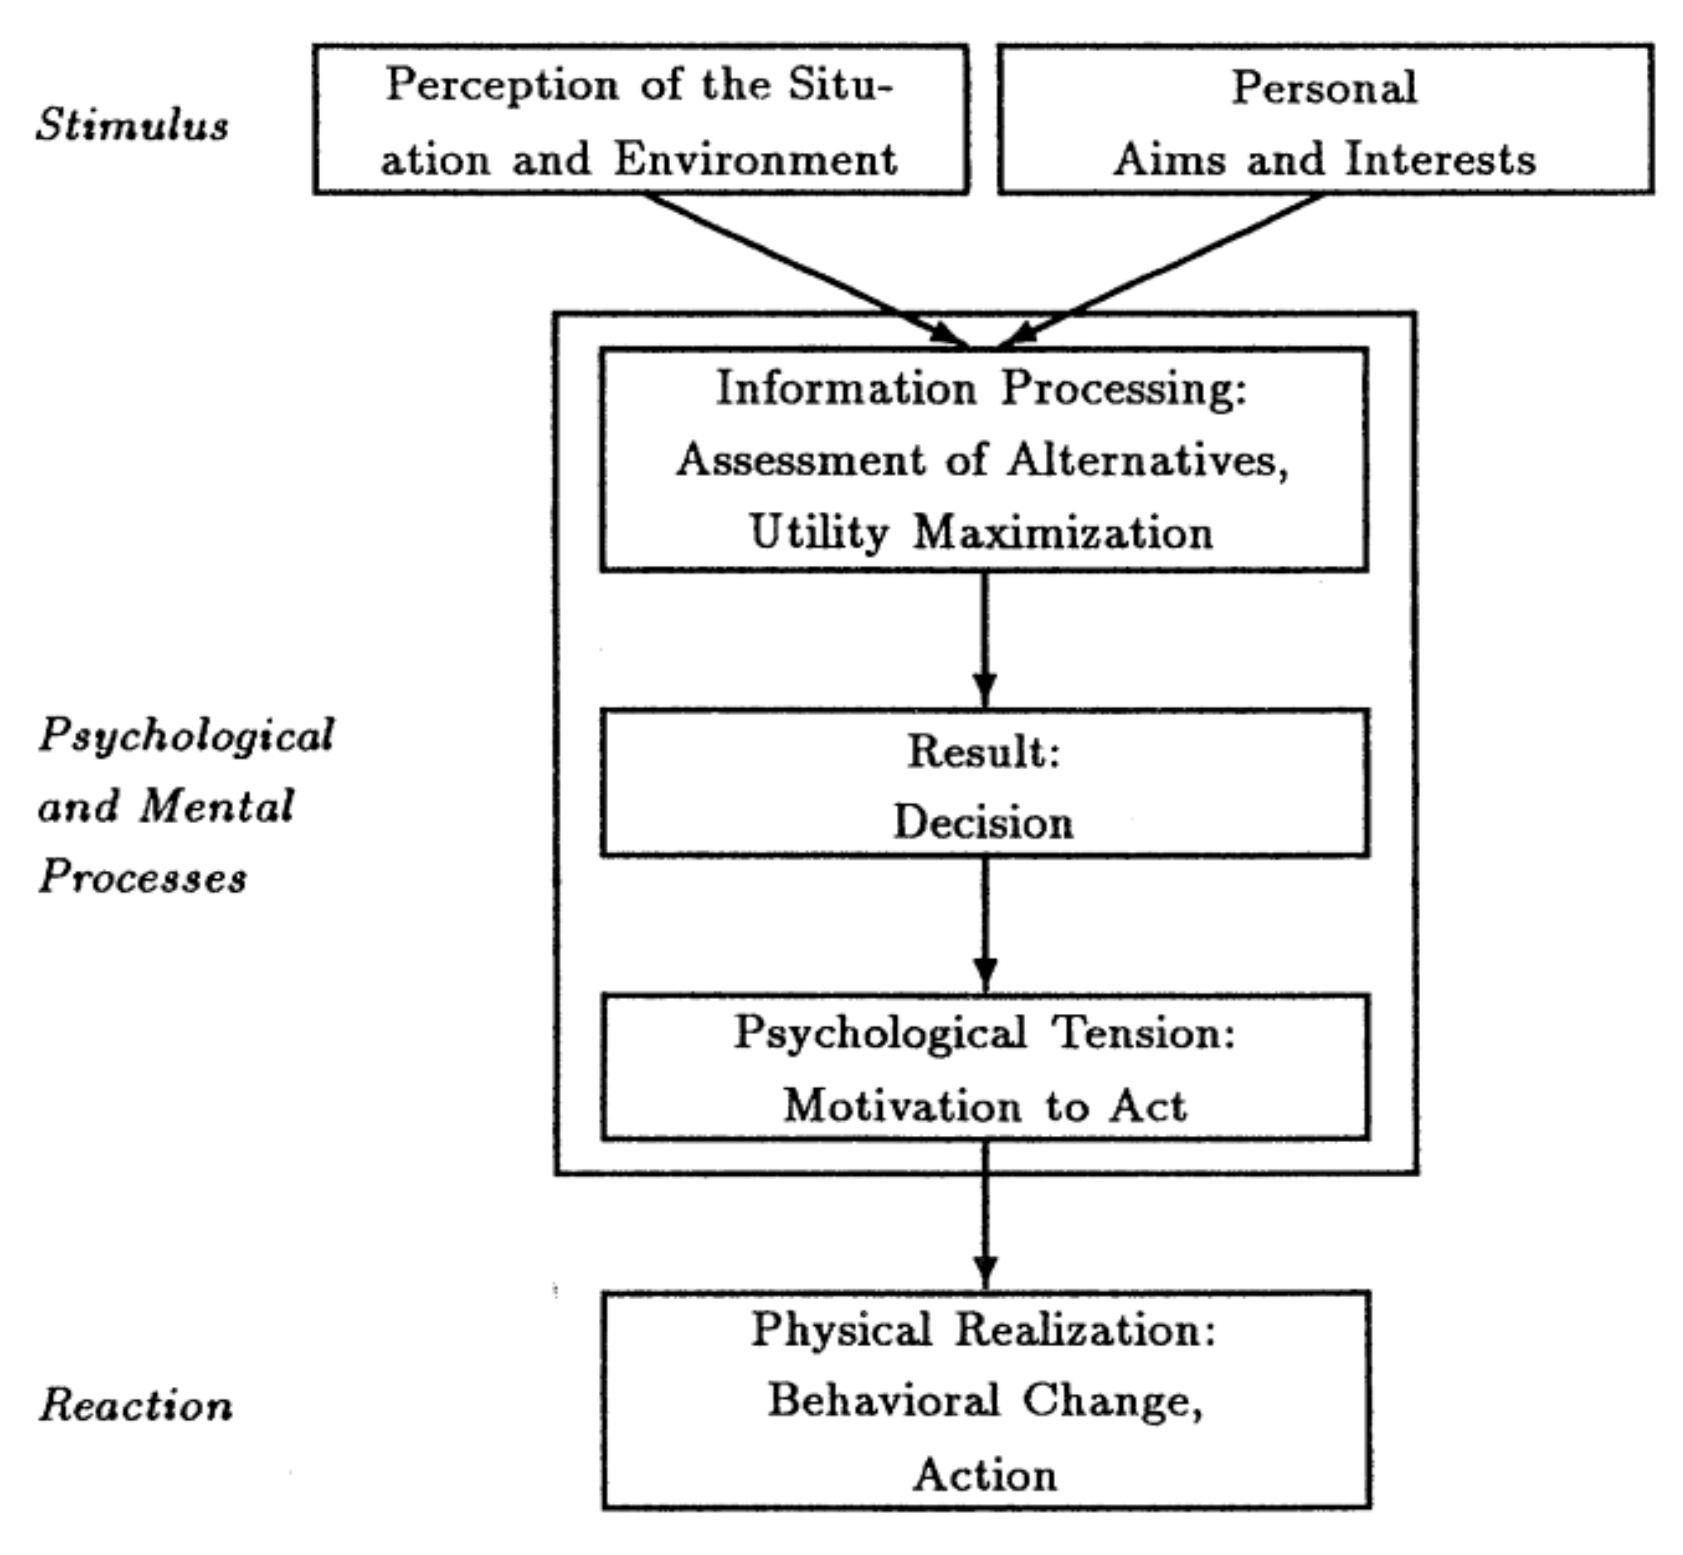
\includegraphics[width=1\linewidth]{images/helbingSocialForceConceptScheme.png}
  \caption{sequence of actions in the social force concept, taken from \cite{helbing_social_1995}}
  \Description{sequence of actions in the social force concept}
  \label{fig:helbingSchema}
\end{figure}
Fig. \ref{fig:helbingSchema} shows the sequence of actions lead to the a action for the individual crowd agent, which leads back to research done by Lewin \cite{lewin_field_1951}. The Stimulus is used as an trigger like someone is blocking the way, this results in the process of handling the situation which creates an motivation to act and in the final form a reaction which is carried out. This concept can be applied to all situations, \cite{helbing_social_1995} however describes a model for common situation which are decided usually automatically and intuitively by the person. The idea is to describe the pedestrian movement indirectly through describing the external forces which affects the agent. 
Helbings social force model uses 3 main effects for the model:
\begin{enumerate}
    \item the goal for the person is to reach some sort of target destination as easy as possible, usually the fasted route.
    \item "repulsive effect", the pedestrian wants to "keep a certain distance from other pedestrians that depends on the pedestrian density and the desired speed". In addition the pedestrian also want to keep distance to borders.  
    \item "attracted effect", the pedestrians " are sometimes attracted by other persons (friends, street artists, etc.) or objects (e.g., window displays)."
\end{enumerate}
In the paper all effects are described in detail with mathematically equations, these are not displayed here for reasons of clarity. The result movement decision is the sum of all effects plus a fluctuation term for situations where two alternatives are rated equally. Simulations with this models shows 
\begin{quote}
    "(i) the development of lanes consisting of pedestrians who walk into the same direction and (ii) oscillatory changes of the walking direction at narrow passages."
\end{quote}
This behaviour can also be observed in real world scenarios. 

\subsubsection{Simulating dynamical features of escape panic}\cite{helbing_simulating_2000} on the other hand there is also a need for simulating pedestrians in a panic situation, a common example are evacuation simulations.
There are a number of reasons for a panic reaction in a crowd, unexpected actions like an loud gun shot or a fire are a common reasons most people would think about. But also expected situations like the race for a limited amount of resources (tickets, seats, toilet paper in the corona crisis)  and situations without any cause at all can cause a crowd panic. These panic reactions often lead to tragic events and cause harm to people seen for example on the panic at the loveparade 2010 \cite{dumbs_massenpanik_2010} . That events also show that the reaction of the individual agent is way more complex in a panic situation than under normal circumstances, this makes the development for a crowd behavioural model of course difficult, in addition the paper also states that there is not enough suitable data to the their panic model. 

The paper gives an definition of features of a panic situation, some of them are (1) People move faster than normal (2) People start pushing and so on. They use these features to construct a behaviour model based on the "generelized force model"\cite{hindsley_investigation_1986}
\begin{quote}
"We assume a mixture of psychological and physical forces influencing the behaviour in a crowd"
\end{quote}
Again the mathematically details are not displayed here for reasons of clarity. They also ran a number of different tests with the model, the results show the following:
\begin{itemize}
\item "Transition to in-coordination due to clogging" In a situation where the crowd want to exit an area trough a small gap, the number of people leaving get smaller when the velocity of the crowd increases.
\item "Faster-is-slower effect due to impatience", clogging can appear also when there is a wider gap in the escape route. 
\item "Mass behaviour" Here the goal was to leave a room with smoke in it, results showed that the quickest evacuation would be possible when there is a equal mixture of individualistic and herding behaviour. 
\end{itemize}
In their model they have a "panic parameter" which allows to adjust the "amount" of panic in comparison to a normal daily situation. Because the results are also observed in real crowd panics, their model is often used as a base for a number of other evacuation simulation papers. \cite{braun_simulating_2005} \cite{zheng_modeling_2009}

\section{Application Areas}

As the research field for crowd simulation is already wide spread over multiple science fields and communities the resulting application areas are of course too. The applications can be roughly grouped by the key areas mentioned before \ref{chap:key_areas}. 

\subsection{realism focused simulation }

In the area of realism focused simulation pedestrian and traffic simulation plays a big role, as these are used to simulate large urban areas. There are a number of commercial available software for similar use-cases like simulating the crowd flow on events, public transport buildings, airports and even cruise ships and whole city districts. They often feature come with extended features which goes beyond the crowd simulation like heat-maps, smoke simulation, integration for 3D models and other CAD applications, recording and playback and so on. The customers for these applications are public transport companies, architectural offices, event organizers and the public governance sector. The simulation allows them to reduce costs in the planning phase and optimize their infrastructure, simulation of the evacuation times required is also a market for these applications.  Some example Applications are "Pedestrian Dynamics®" \cite{pedestrian_dynamics_pedestrian_2020}, "MassMotion"  \cite{mediaworks_pedestrian_2020} and "Anylogic" \cite{anylogic_website}

\begin{figure}[h]
  \centering
  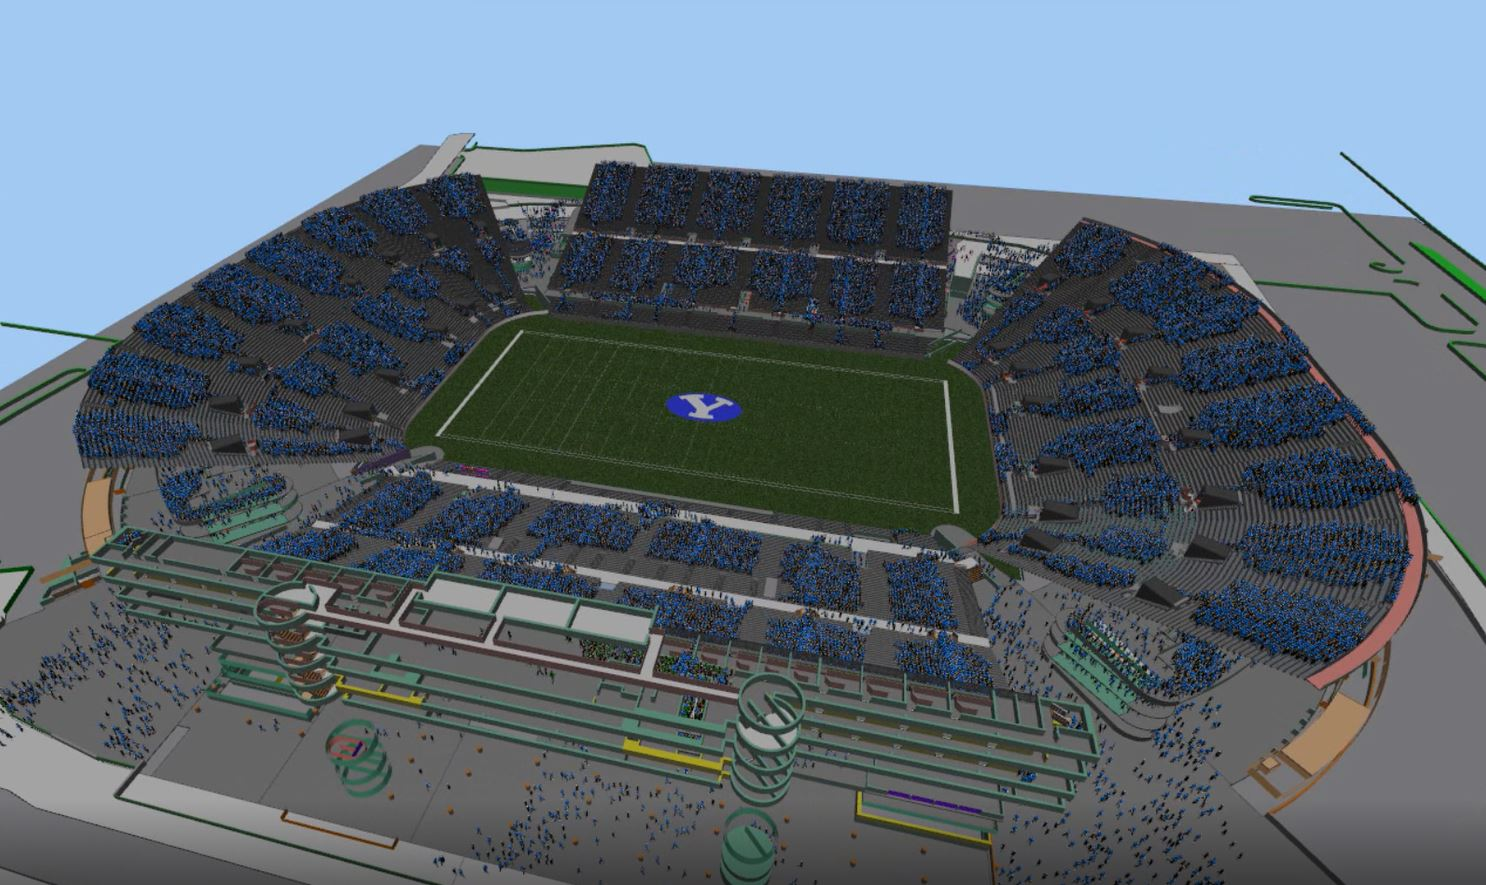
\includegraphics[width=1\linewidth]{images/PedestrianDynamicsStadionExample.png}
  \caption{example visualization of a pedestrian flow in the commercial program "Pedestrian Dynamics®",  taken from \cite{pedestrian_dynamics_pedestrian_2020}}
  \Description{example visualization of a pedestrian flow in a stadium}
  \label{fig:stadionEvacuationExample}
\end{figure}

Although the visual presentation is not the focus on these applications it does not necessarily have to look simply. Some of the introduced commercial tools also have export functions for the generated behaviour especially the movement, these exports can be used later to produce visual appealing videos in 3D applications like "3ds Max" as a demo of Jordan Lynam shows us. \cite{lynamJordan_viissim_3ds_max}

\subsection{High quality focused simulation}

On the other hand we have the visual focused applications, in comparison to the realism focused simulation application the amount of public available applications and research is rare and hard to find. The reason for this is that, especially the applications used for movies, are highly proprietary and not published. Most of the time information is only available in the form of making-of documentaries, interviews and CGI trailers. 
However the foundation, these applications are based on, is usually public available in the form of scientific papers. The challenges these applications are confronted with are strongly influenced by the crowd rendering research field, especially in games as these require real-time simulations. \cite{thalmann_crowd_2013}

\subsubsection{Movies}

There are multiple benefits of crowd simulation for movies and other types of creative video content, an nearly endless amount of possible scenes and shots can be created, for example an huge battle or a populated city. Some scenes would just not be able to animate manually with CGI not to mention to hire an amount of actors. In comparison to the realism focused applications, simulations on movies does not have the strong urge of proper continuous crowd behavior as movies are grouped in shots where the viewer often don't see the same part of the crowd for a longer time period. Lastly creative content obviously don't always want realistic crowd animators see crowd animation more as a tool for controlling large crowds, so the research field for manipulation of crowds is also an important aspect on movie crowd simulation,  examples are \cite{kim_interactive_2014} \cite{ulicny_crowdbrush_2004}

In the recent movie "THE HOBBIT: Battle of Five Armies" there were  two types of crowd simulation tools used, "Massive", one of the most advanced non-real-time simulation tools \cite{massive_website} , for rendering the final scenes in post production, which at this scales requires render farms and weeks or even months to finish, therefore a second tool "army-manager" was used earlier in the production as this could render much faster and allowed the visual effects team to plan their shots and get a draft of the final simulation them. \cite{wired_hobbit_doku}

On the example of the movie "World War Z" we can also see that the simulations are often combined with a database of motion captures scenes, we already saw that approach at some papers (TODO: cite paper), and rigid body physics. In addition the "Alice" program which is used to simulate the zombie crowds, uses an microscopic based model where each agent is simulated by given rules and attributes, which we already know from a lot of papers. \cite{wired_worldwarz_doku} 

An other commercial software for CGI crowds is "Golaem" \cite{golaem_website}. This software can be purchased for individual projects and is therefore used for movies with a smaller budget, commercials or other short CGI clips in need for crowds, which can't afford to develop an own software tool, but it is also used for big budget production of example in "Game of Thrones" \cite{golaem_got_vid}
\cite{thalmann_crowd_2013}
\subsubsection{Games}

As games and other interactive media are real-time simulations they have limited capabilities for costly simulations, so crowd simulations are not so common in today's games. One game genre that uses them are real-time strategy games like Total War \cite{total_war_website}, where the crowd simulation can also have an effect on the gameplay and not only used to render visually appealing large crowds. 
Many approaches for real time simulation is used one common used technique is the LOD (level of detail) for the rendering of the crowd and also for the simulation it self. However LOD is more complex when used on the actual crowd behaviour simulation than on the crowd rendering itself, there is always the danger of getting an wrong simulated world when the simulation detail level is too low. Another common used trick is to render one simulated agent as multiple persons to simulate a crowd. Lastly as games are usually run on a powerful GPU, real time crowd simulation can also benefit from that, especially the rendering part is good manageable by the GPU. 

An example of what can be done with various optimization is "Ultimate Epic Battle Simulator" \cite{ultimeEpicBattleSim_video} , which is basically a big real-time crowd simulation sandbox. They manage to simulate path tracing on up to ten thousands of individual soldiers in real time . 
\begin{quote}
"The algorithm is a highly optimized version of A*.  The memory is shared, but the paths are not." \cite{ultimeEpicBattleSim_video}
\end{quote} This example shows that crowd simulation at games comes with a big trade off for performance. 

%%
%% The acknowledgments section is defined using the "acks" environment
%% (and NOT an unnumbered section). This ensures the proper
%% identification of the section in the article metadata, and the
%% consistent spelling of the heading.
\begin{acks}
To Robert, for the bagels and explaining CMYK and color spaces.
\end{acks}

%%
%% The next two lines define the bibliography style to be used, and
%% the bibliography file.
\bibliographystyle{ACM-Reference-Format}
\bibliography{literaturVerzeichnis}

%%
%% If your work has an appendix, this is the place to put it.
\appendix

\end{document}
\endinput
%%
%% End of file `sample-xelatex.tex'.
